\chaptertitlepage{System Design}

This chapter translates the methodology into a layered software system: presentation (HTML/CSS/Jinja), application (Flask routes), inference service (lazy loading, locking, ensemble), model artefacts (\texttt{weights/}), and an offline training pipeline under \texttt{training/}.

\section{System Architecture}

The inference path is layered as follows: user upload is received by Flask routes, validated by the chest X-ray gate, scored by \texttt{predict\_all()} in \texttt{predictors.py} across EfficientNetB3, DenseNet121, and the Custom CNN, then aggregated by soft-voting ensemble before the result page shows probability bars and agreement status.

\begin{figure}[H]
\centering
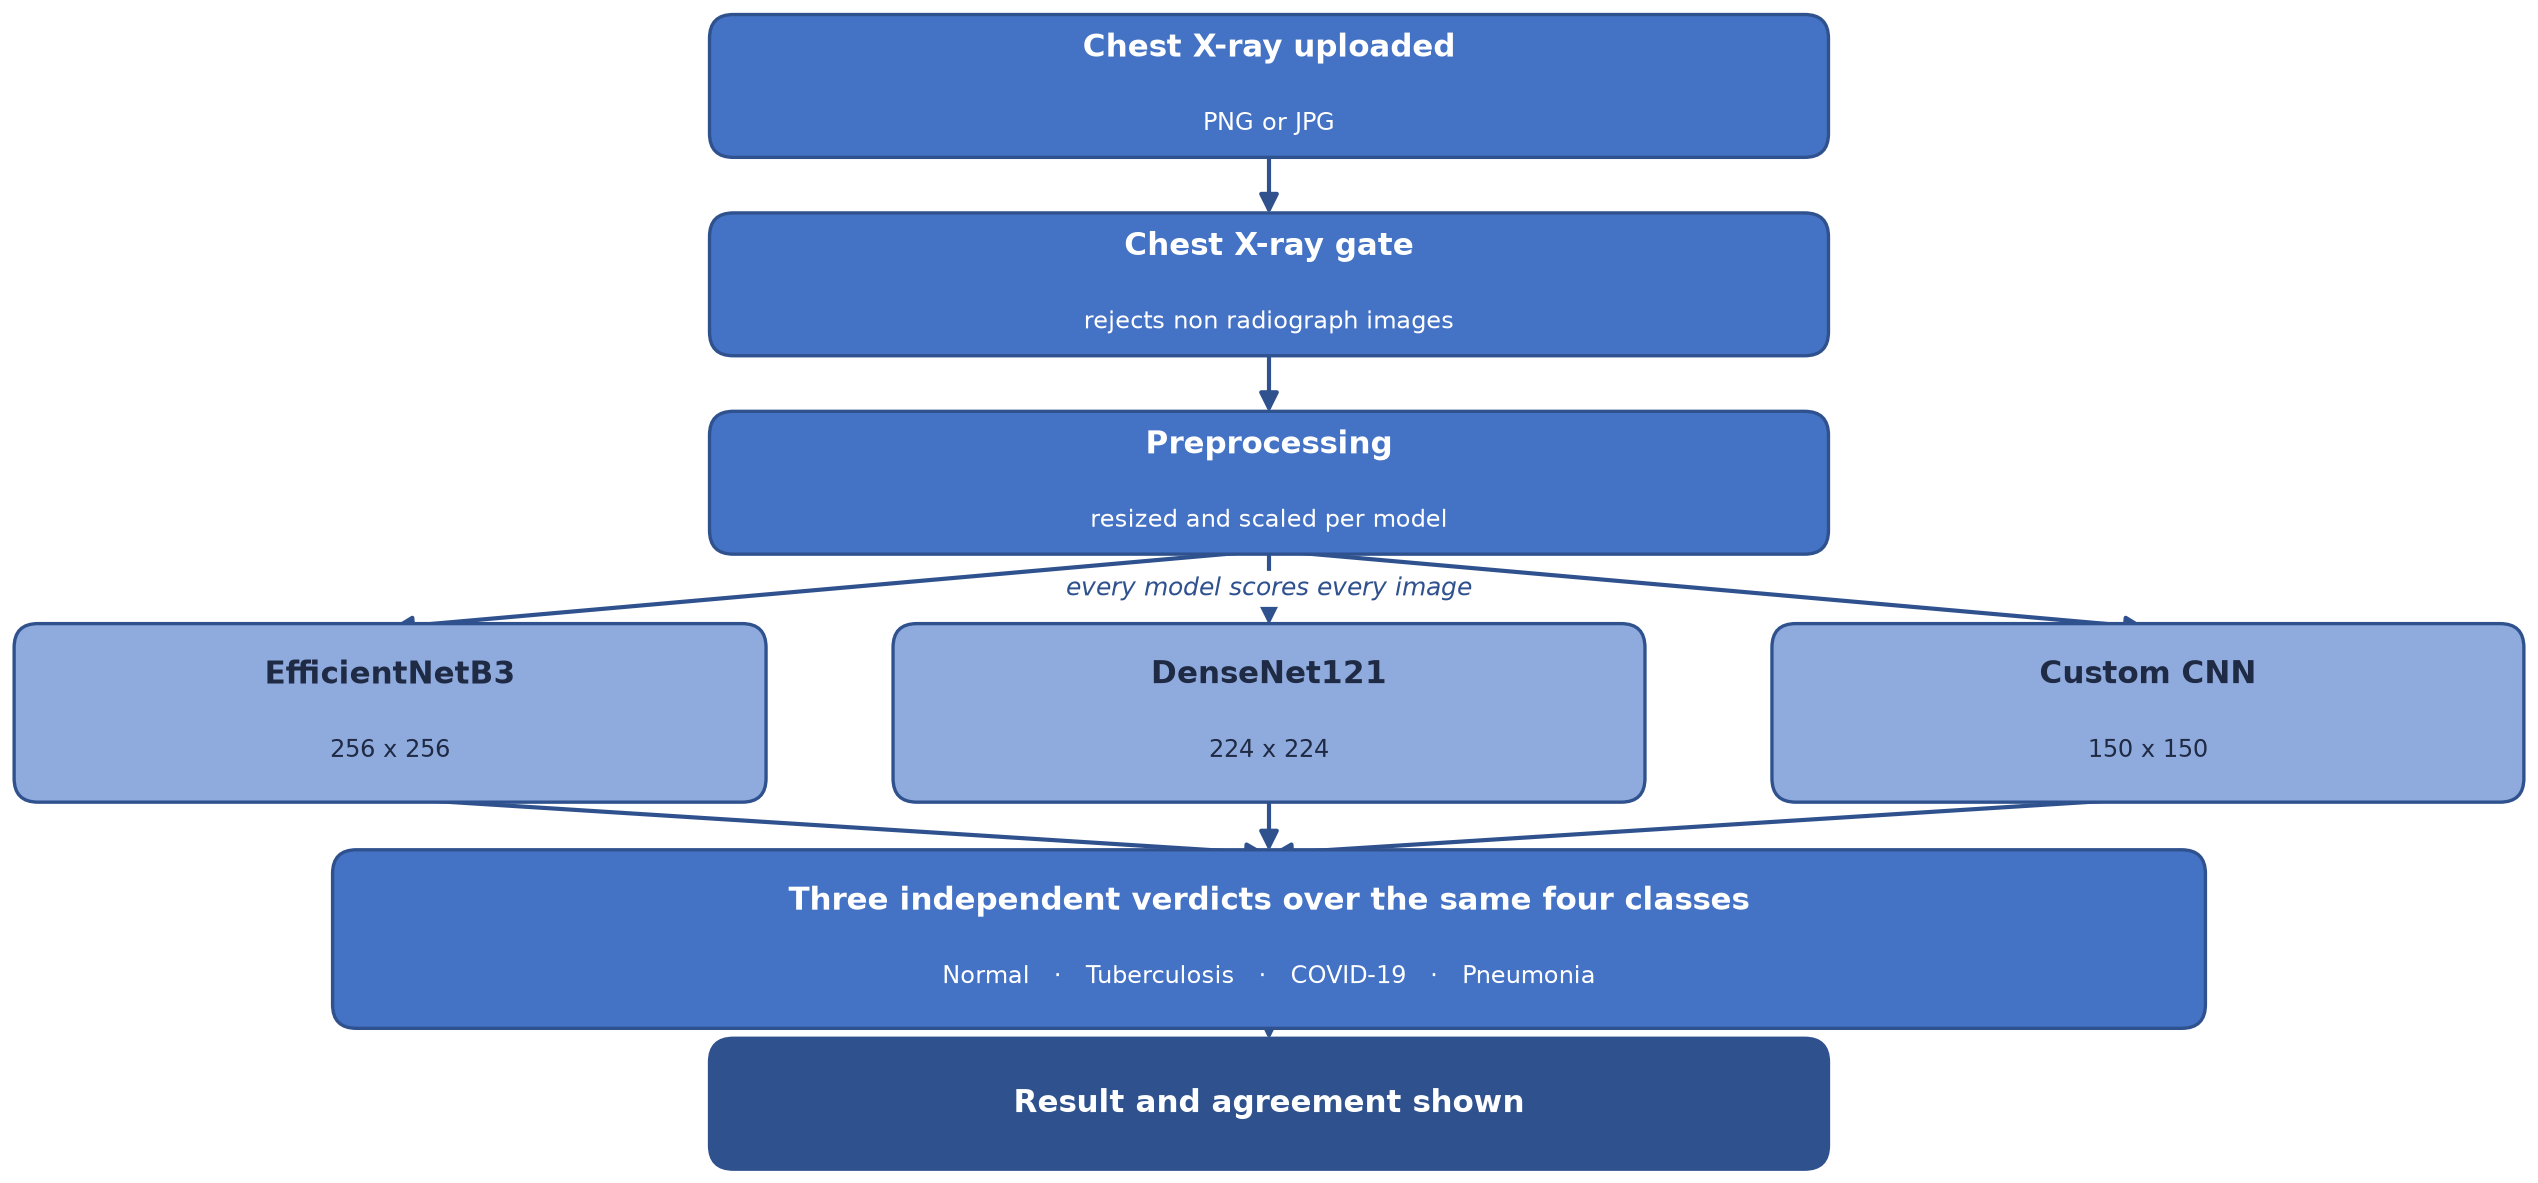
\includegraphics[width=0.92\textwidth]{images/diagrams/system_architecture.png}
\caption{High-level inference flow for the unified four-class web application}
\label{fig:sys-arch-flow}
\end{figure}

Every upload is scored by every trained four-class model under the locked label order Normal, Tuberculosis, COVID-19, Pneumonia. Soft voting averages probability vectors. Legacy single-disease \texttt{.h5} files are refused if the output width is not four; missing weights are reported without crashing the server.

\begin{table}[H]
\centering
\caption{Model integration overview}
\label{tab:model-integration}
\small
\begin{tabular}{@{}llcc@{}}
\toprule
\HeaderRow \Head{Architecture} & \Head{Output} & \Head{Input} & \Head{Interface} \\
\midrule
EfficientNetB3 & 4-class softmax & $256\times256$ & Flask ensemble \\
\ZebraRow DenseNet121 & 4-class softmax & $224\times224$ & Flask ensemble \\
Custom CNN & 4-class softmax & $150\times150$ & Flask ensemble \\
\bottomrule
\end{tabular}
\end{table}


\section{Functional Requirements}

\begin{itemize}
    \item \textbf{FR1:} Accept PNG/JPG/JPEG uploads (maximum 16\,MB).
    \item \textbf{FR2:} Validate likely chest radiographs; allow forced override with warning.
    \item \textbf{FR3:} Run every available 4-class model on the same image.
    \item \textbf{FR4:} Display per-class probabilities per model.
    \item \textbf{FR5:} Compute and display soft-voting ensemble and agreement.
    \item \textbf{FR6:} Show clear errors if weights are missing or have wrong output width.
    \item \textbf{FR7:} Provide offline training scripts to rebuild weights from the manifest.
\end{itemize}

\section{Non-Functional Requirements}

\begin{itemize}
    \item \textbf{NFR1 Reproducibility:} Fixed seed and committed manifest policy.
    \item \textbf{NFR2 Usability:} Single upload; no model picker required.
    \item \textbf{NFR3 Robustness:} Multi-stage rejection of non-X-ray uploads.
    \item \textbf{NFR4 Consistency:} Train/serve preprocessing alignment.
    \item \textbf{NFR5 Maintainability:} Shared \texttt{CLASSES} order in \texttt{training/common.py}.
    \item \textbf{NFR6 Safety messaging:} Explicit research-only / non-clinical disclaimer.
\end{itemize}

\section{Tools and Technologies Used}

Python (3.9+/3.11 recommended for modern TensorFlow), TensorFlow and Keras, OpenCV, Flask and Werkzeug, NumPy, scikit-learn (evaluation), Matplotlib and Seaborn (figures), HTML/CSS, and Git. Training prefers a capable GPU machine; CPU inference is possible but slower. Key folders: \path{training/}, \path{Frontend/}, \path{weights/}, and the three public dataset trees documented in Chapter~3.

\section{Chest X-Ray Validation Gate}

\begin{enumerate}
    \item \textbf{Monochrome/tint:} grayscale or single-tint films (blue-tinted displays allowed).
    \item \textbf{Radiograph envelope:} intensity, entropy, midtones, aspect, symmetry, and related statistics; one violation forgiven.
    \item \textbf{Anatomy veto:} reject only if both bright central-column cues and bilateral symmetry cues are absent.
\end{enumerate}

\begin{figure}[H]
\centering
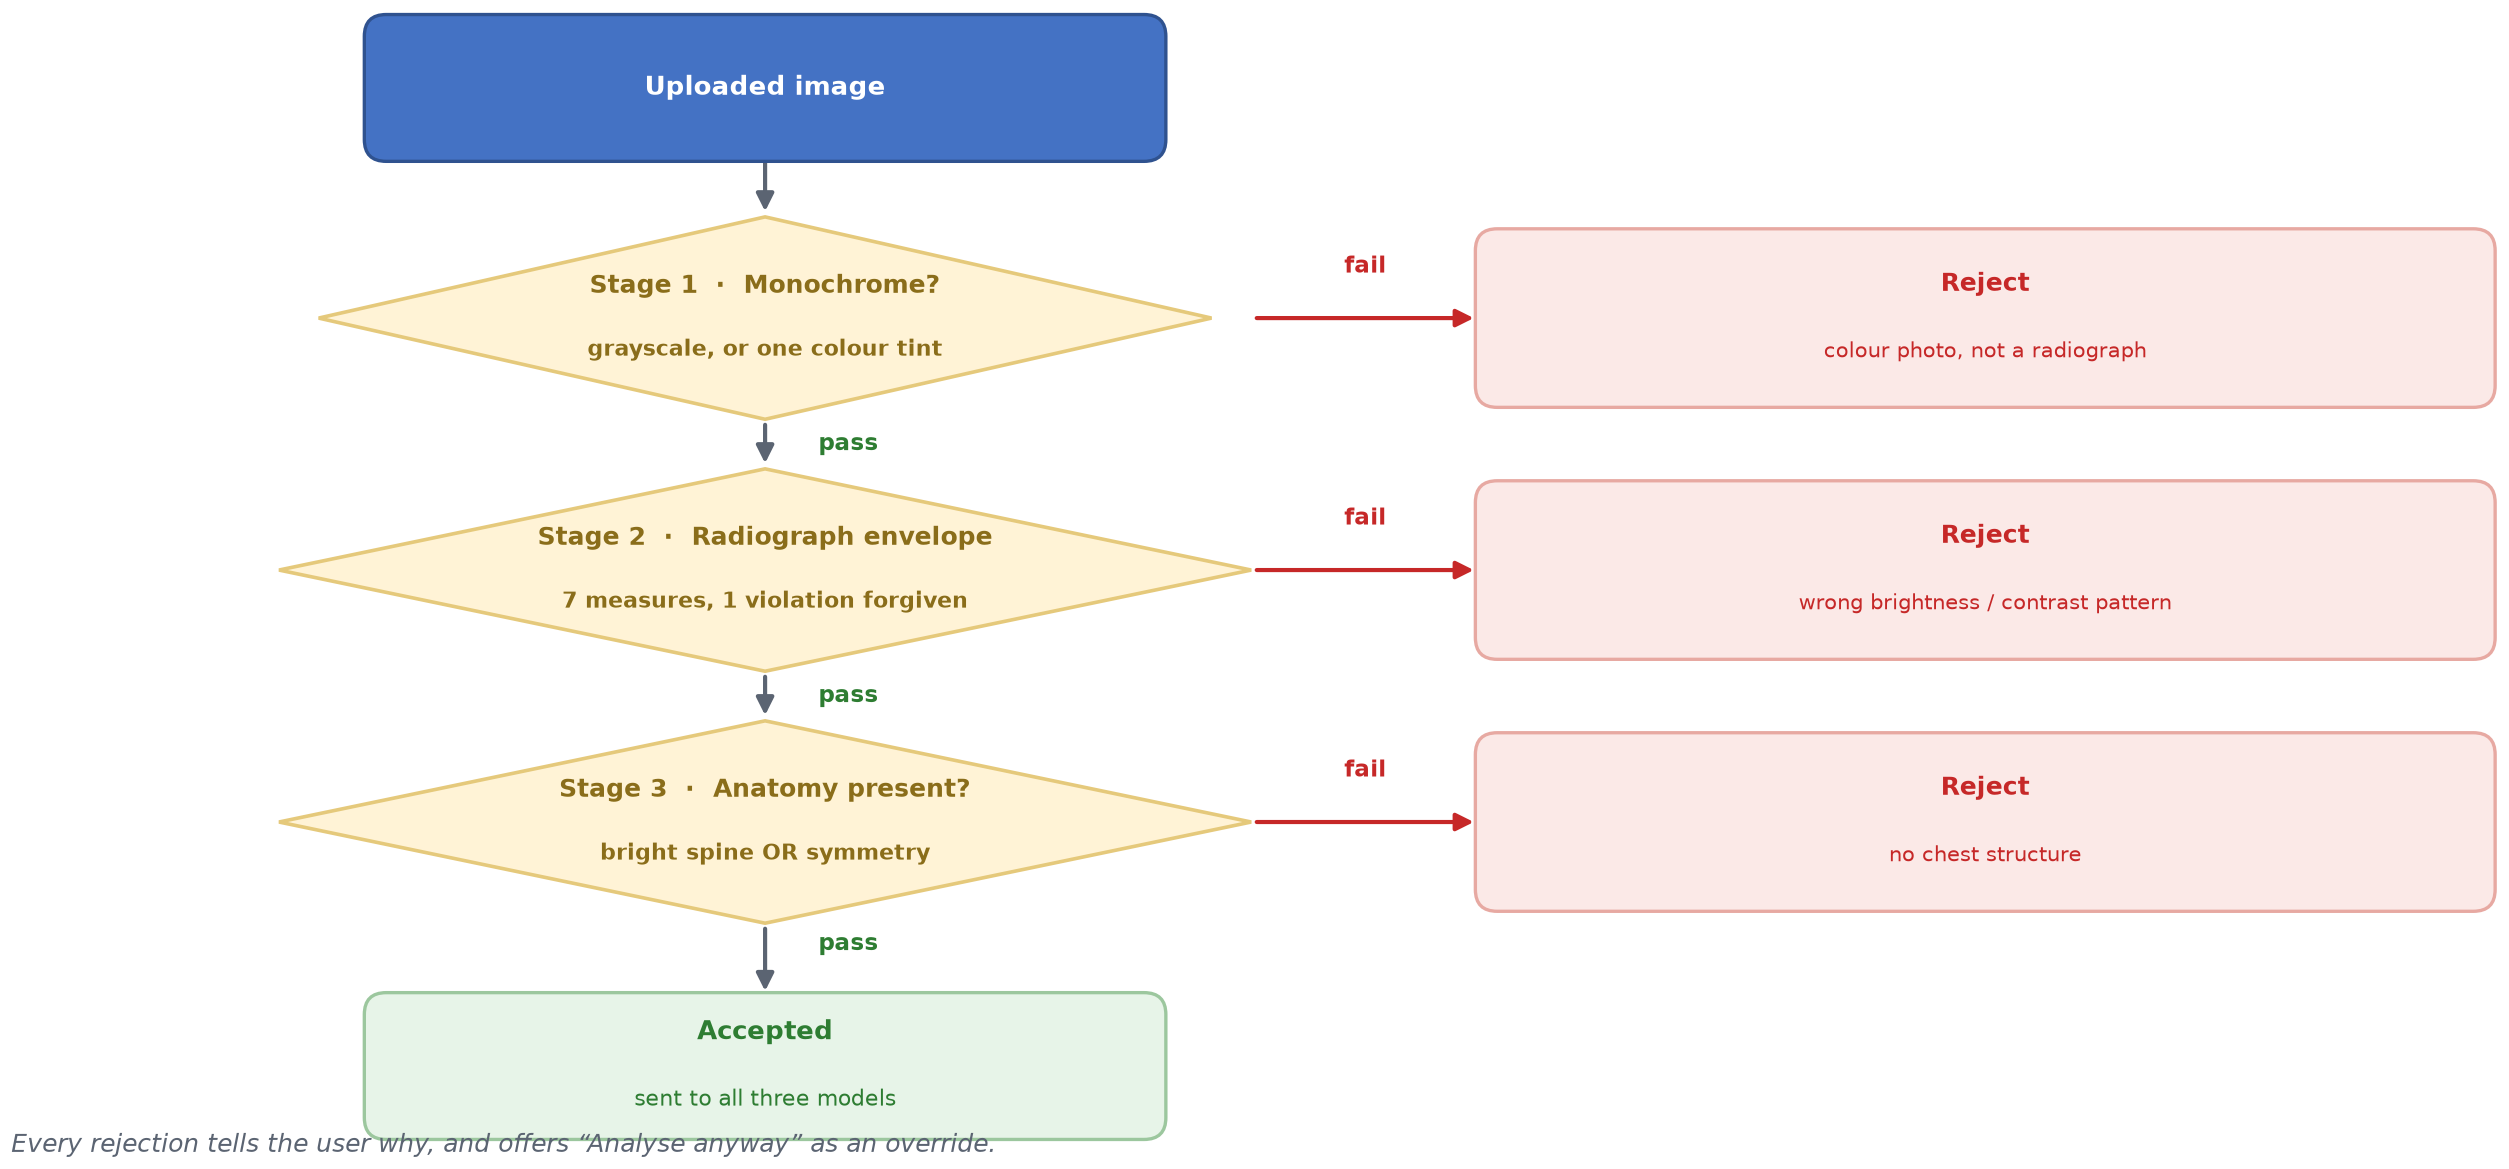
\includegraphics[width=0.92\textwidth]{images/diagrams/xray_gate_pipeline.png}
\caption{Three-stage chest X-ray validation gate with optional forced analysis}
\label{fig:xray-gate}
\end{figure}

On a labelled set of 351 real radiographs versus 106 non-X-rays, the gate accepted 100\% of real films and rejected approximately 77\% of non-X-rays (previous monochrome-only gate $\sim$21\%). Rejection reasons are shown; Analyse anyway is protected against path traversal.

\section{Application Flow and User Interface}

Home lists model readiness; the upload form accepts a radiograph; results show probability bars, class blurbs, ensemble verdict, agreement, and a forced-analysis warning when used. Figures~\ref{fig:web-upload-ui} and~\ref{fig:web-validation} show upload and rejection UI; Chapter~5 presents consensus result screenshots for TB, COVID-19, and pneumonia demos.

\begin{figure}[H]
\centering
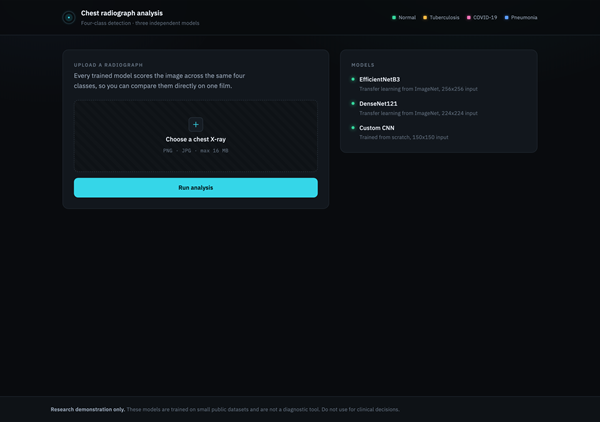
\includegraphics[width=0.92\textwidth]{images/ui_upload.png}
\caption{Flask upload interface for four-class multi-model chest radiograph analysis}
\label{fig:web-upload-ui}
\end{figure}

\begin{figure}[H]
\centering
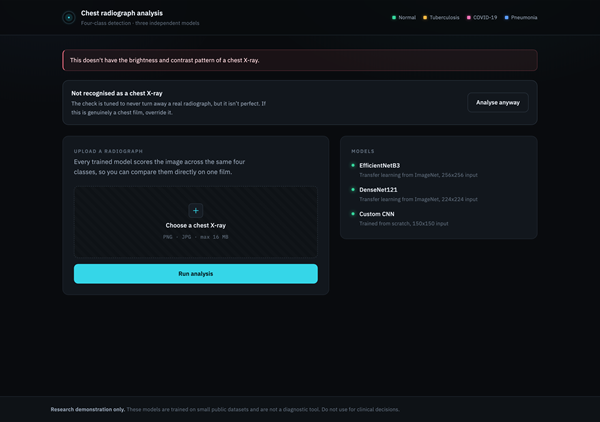
\includegraphics[width=0.92\textwidth]{images/ui_gate_reject.png}
\caption{Chest X-ray validation gate rejection with Analyse anyway option}
\label{fig:web-validation}
\end{figure}

\begin{table}[H]
\centering
\caption{Flask application components}
\label{tab:flask-components}
\small
\begin{tabular}{@{}P{2.4cm}P{4.0cm}P{5.5cm}@{}}
\toprule
\HeaderRow \Head{Component} & \Head{Location} & \Head{Purpose} \\
\midrule
Web Framework & Flask & Routes and templates \\
\ZebraRow Inference & \path{Frontend/predictors.py} & Gate, lazy load, ensemble \\
Shared constants & \texttt{training/common.py} & Class order, preprocess \\
\ZebraRow Weights & \texttt{weights/*.keras} & 4-class models \\
\bottomrule
\end{tabular}
\end{table}

\section{Train/Serve Consistency}

Inference mirrors training decode with bilinear resize and the same \texttt{preprocess\_input} or $/255$ rescale. The \texttt{CLASSES} index order is shared across training, evaluation, and the UI. Non-four-class weight files are refused.

\section{Summary}

The system turns the methodology into a research demo that people can use. It checks uploads before they reach the models, scores every image with all three models, combines them by soft voting, and preprocesses images the same way in the live application as in training.
